% Options for packages loaded elsewhere
\PassOptionsToPackage{unicode}{hyperref}
\PassOptionsToPackage{hyphens}{url}
\documentclass[
  ignorenonframetext,
]{beamer}
\newif\ifbibliography
\usepackage{pgfpages}
\setbeamertemplate{caption}[numbered]
\setbeamertemplate{caption label separator}{: }
\setbeamercolor{caption name}{fg=normal text.fg}
\beamertemplatenavigationsymbolsempty
% remove section numbering
\setbeamertemplate{part page}{
  \centering
  \begin{beamercolorbox}[sep=16pt,center]{part title}
    \usebeamerfont{part title}\insertpart\par
  \end{beamercolorbox}
}
\setbeamertemplate{section page}{
  \centering
  \begin{beamercolorbox}[sep=12pt,center]{section title}
    \usebeamerfont{section title}\insertsection\par
  \end{beamercolorbox}
}
\setbeamertemplate{subsection page}{
  \centering
  \begin{beamercolorbox}[sep=8pt,center]{subsection title}
    \usebeamerfont{subsection title}\insertsubsection\par
  \end{beamercolorbox}
}
% Prevent slide breaks in the middle of a paragraph
\widowpenalties 1 10000
\raggedbottom
\AtBeginPart{
  \frame{\partpage}
}
\AtBeginSection{
  \ifbibliography
  \else
    \frame{\sectionpage}
  \fi
}
\AtBeginSubsection{
  \frame{\subsectionpage}
}
\usepackage{iftex}
\ifPDFTeX
  \usepackage[T1]{fontenc}
  \usepackage[utf8]{inputenc}
  \usepackage{textcomp} % provide euro and other symbols
\else % if luatex or xetex
  \usepackage{unicode-math} % this also loads fontspec
  \defaultfontfeatures{Scale=MatchLowercase}
  \defaultfontfeatures[\rmfamily]{Ligatures=TeX,Scale=1}
\fi
\usepackage{lmodern}
\ifPDFTeX\else
  % xetex/luatex font selection
\fi
% Use upquote if available, for straight quotes in verbatim environments
\IfFileExists{upquote.sty}{\usepackage{upquote}}{}
\IfFileExists{microtype.sty}{% use microtype if available
  \usepackage[]{microtype}
  \UseMicrotypeSet[protrusion]{basicmath} % disable protrusion for tt fonts
}{}
\makeatletter
\@ifundefined{KOMAClassName}{% if non-KOMA class
  \IfFileExists{parskip.sty}{%
    \usepackage{parskip}
  }{% else
    \setlength{\parindent}{0pt}
    \setlength{\parskip}{6pt plus 2pt minus 1pt}}
}{% if KOMA class
  \KOMAoptions{parskip=half}}
\makeatother
\usepackage{longtable,booktabs,array}
\usepackage{caption}
\captionsetup[table]{skip=6pt}
\newcounter{none} % for unnumbered tables
\usepackage{calc} % for calculating minipage widths
\usepackage{caption}
% Make caption package work with longtable
\makeatletter
\def\fnum@table{\tablename~\thetable}
\makeatother
\usepackage{graphicx}
\makeatletter
\newsavebox\pandoc@box
\newcommand*\pandocbounded[1]{% scales image to fit in text height/width
  \sbox\pandoc@box{#1}%
  \Gscale@div\@tempa{\textheight}{\dimexpr\ht\pandoc@box+\dp\pandoc@box\relax}%
  \Gscale@div\@tempb{\linewidth}{\wd\pandoc@box}%
  \ifdim\@tempb\p@<\@tempa\p@\let\@tempa\@tempb\fi% select the smaller of both
  \ifdim\@tempa\p@<\p@\scalebox{\@tempa}{\usebox\pandoc@box}%
  \else\usebox{\pandoc@box}%
  \fi%
}
% Set default figure placement to htbp
\def\fps@figure{htbp}
\makeatother
\setlength{\emergencystretch}{3em} % prevent overfull lines
\providecommand{\tightlist}{%
  \setlength{\itemsep}{0pt}\setlength{\parskip}{0pt}}
% Auto-generated by infrastructure/rendering/_pdf_latex_helpers.py::extract_math_font_preamble.
% Minimal header passed to Pandoc via -H so Beamer slides pick up the same math font
% as the combined-PDF path. Adjust the manuscript's preamble.md to change the font globally.
\usepackage{unicode-math}
\setmathfont{latinmodern-math.otf}

% Manuscript macro/package fallbacks (newcommand -> providecommand).
% Core mathematics
\usepackage{amsmath}
\usepackage{amssymb}
% Document layout
% Tables
\usepackage{booktabs}
% Algorithm typesetting (for pseudocode in §2 Methodology)
% Code listings
\usepackage{listings}
% Typography and formatting
% Cross-references and citations
% ── Unicode-capable mono font for code listings ──────────────────────
% JuliaMono (TeX Live 2026) covers the full math/Greek glyph set used in
% scientific code blocks; the default lmmono lacks \alpha/\mu/\partial/\nabla.
%
% The hardcoded TeX Live 2026 path below is portable to most macOS / Linux
% TeX Live installs that placed JuliaMono under the default texmf-dist path.
% If your TeX Live version differs (e.g., 2025, 2027) or your distribution
% installs fonts elsewhere, comment out the explicit Path = line — fontspec
% will then search the system font path. If JuliaMono is not installed at
% all, comment out the whole block; xelatex falls back to lmmono with
% reduced Unicode coverage but the document still compiles.
% Math font for unicode-math: Latin Modern Math (TeX Live) has full BMP
% coverage including U+2223 (\mid), U+226A/226B (\ll/\gg), and the Greek/
% blackboard letters used in equations. Without an explicit \setmathfont,
% unicode-math falls back to lmroman text font which lacks several glyphs
% and emits "Missing character" warnings on every \mid in math mode.

% Slide layout defaults for warning-clean scientific decks.
\usepackage{etoolbox}
\IfFileExists{xurl.sty}{\usepackage{xurl}}{}
\IfFileExists{seqsplit.sty}{\usepackage{seqsplit}}{\newcommand{\seqsplit}[1]{#1}}
\protected\def\breakseq#1{\seqsplit{#1}}
\protected\def\breaktt#1{\begingroup\ttfamily\seqsplit{#1}\endgroup}
\setlength{\emergencystretch}{6em}
\tolerance=5000
\hbadness=10000
\hfuzz=1pt
\setlength{\tabcolsep}{2pt}
\AtBeginEnvironment{longtable}{\tiny\renewcommand{\arraystretch}{0.86}\setlength{\tabcolsep}{1pt}}
\AtBeginEnvironment{tabular}{\tiny\renewcommand{\arraystretch}{0.86}\setlength{\tabcolsep}{1pt}}
\AtBeginEnvironment{equation}{\tiny}
\AtBeginEnvironment{equation*}{\tiny}
\AtBeginEnvironment{align}{\tiny}
\AtBeginEnvironment{align*}{\tiny}
\AtBeginEnvironment{itemize}{\footnotesize}
\AtBeginEnvironment{enumerate}{\footnotesize}
\AtBeginEnvironment{description}{\footnotesize}
\setbeamerfont{caption}{size=\tiny}
\setbeamerfont{caption name}{size=\tiny}
\setbeamerfont{normal text}{size=\small}
\setbeamerfont{frametitle}{size=\small}
\setbeamerfont{section title}{size=\footnotesize}
\setbeamerfont{subsection title}{size=\footnotesize}
\setbeamertemplate{section page}{%
  \centering
  \begin{beamercolorbox}[sep=12pt,center,wd=\paperwidth]{section title}
    \parbox{0.86\paperwidth}{\centering\usebeamerfont{section title}\insertsection\par}
  \end{beamercolorbox}
}
\setbeamertemplate{subsection page}{%
  \centering
  \begin{beamercolorbox}[sep=8pt,center,wd=\paperwidth]{subsection title}
    \parbox{0.86\paperwidth}{\centering\usebeamerfont{subsection title}\insertsubsection\par}
  \end{beamercolorbox}
}
\setlength{\abovecaptionskip}{2pt}
\setlength{\belowcaptionskip}{0pt}

% Natbib and cross-reference fallbacks — slides don't load natbib
% or cleveref, but combined-PDF manuscript prose may emit these
% commands. The fallback renders citations as a bracketed key list
% and cross-references as detokenized labels so slides don't fail on
% undefined control sequences or raw underscores. \providecommand is
% a no-op if packages load later.
\providecommand{\citep}[1]{[#1]}
\providecommand{\citet}[1]{#1}
\providecommand{\citealp}[1]{#1}
\providecommand{\citeauthor}[1]{#1}
\providecommand{\citeyear}[1]{#1}
\providecommand{\cref}[1]{\texttt{\detokenize{#1}}}
\providecommand{\Cref}[1]{\texttt{\detokenize{#1}}}
\providecommand{\crefrange}[2]{\texttt{\detokenize{#1}}--\texttt{\detokenize{#2}}}
\providecommand{\Crefrange}[2]{\texttt{\detokenize{#1}}--\texttt{\detokenize{#2}}}
\providecommand{\paragraph}[1]{\textbf{#1}\ }

\newtheorem{proposition}{Proposition}
\newtheorem{hypothesis}{Hypothesis}
\newtheorem{remark}[theorem]{Remark}
\newtheorem{axiom}{Axiom}
\newtheorem{property}{Property}
\usepackage{bookmark}
\IfFileExists{xurl.sty}{\usepackage{xurl}}{} % add URL line breaks if available
\urlstyle{same}
% fallback for those not using the hyperref driver hyperxmp:
\makeatletter
\@ifundefined{xmpquote}{\newcommand{\xmpquote}[1]{#1}}{}
\makeatother
\hypersetup{
  hidelinks,
  pdfcreator={LaTeX via pandoc}}

\author{\texorpdfstring{}{}}
\date{}

\begin{document}

\section{Agentic Authority Architecture: Trust Domains, Controls, and
the Authority Ladder}\label{sec:agentic_authority}

\begin{frame}[allowframebreaks]{The governing rule}
\protect\phantomsection\label{the-governing-rule}
Every architecture in this review answers the exploitation path defined
in sec.~3: harden components so that a compromise
of one does not become a compromise of all. The authorized-misuse path
needs a different instrument. Its governing rule is simple to state and
expensive to honor: \textbf{a component exposed to untrusted input must
not simultaneously hold broad authority over valuable assets.} A browser
parses hostile web content, an agent reads hostile repositories and
documents, a parser processes attacker-shaped files --- and each of
those components is, in the agent era, a candidate for total persuasion
rather than mere compromise. The rule is the classical protection
problem of (Lampson 1974) restated for agents: the question is never
only whether a component can be broken, but who may exercise which
authority through it. It is also the confused-deputy hazard of (Hardy
1988) made continuous: the deputy now reads its instructions from the
\end{frame}

\begin{frame}[allowframebreaks]{The governing rule}
same channel the attacker writes to.

The rule converts directly into architecture. Split the system so that
no component both touches untrusted input and holds broad authority;
place the authority that must exist --- credentials, approvals,
deployment --- behind interfaces too narrow for a persuaded component to
abuse. This section defines that architecture: 7 trust domains, 9
controls that hold regardless of host distribution, and an authority
ladder that separates what an agent may do alone from what requires a
principal outside it.

\end{frame}

\begin{frame}[allowframebreaks]{The governing rule}
\protect\phantomsection\label{def:authority_ladder_order}
The authority ladder orders an agent-initiated change through six rungs;
agent exercise without external authorization is forbidden:
\begin{equation}\protect\phantomsection\label{eq:authority_ladder_order}{\textit{propose} \prec \textit{stage} \prec \textit{authorize} \prec \textit{exercise} \prec \textit{audit} \prec \textit{revoke}}\end{equation}

The section proposes a design; it is not a claim about the defaults of
any distribution reviewed elsewhere in this document. What sharpens the
proposal is that the control vocabulary below is no longer speculative:
the major shipping coding agents now implement versions of these
controls against the same operating-system primitives this review's
server candidates deploy, and the convergences --- and divergences ---
are documented in vendor engineering materials that this section cites
as evidence of mechanism, not as security results (Anthropic 2026b;
OpenAI 2026).
\end{frame}

\begin{frame}[allowframebreaks]{Seven trust domains}
\protect\phantomsection\label{seven-trust-domains}
\end{frame}

\begin{frame}[allowframebreaks]{Seven trust domains}
\begin{longtable}[]{@{}
  >{\raggedright\arraybackslash}p{(\linewidth - 4\tabcolsep) * \real{0.3333}}
  >{\raggedright\arraybackslash}p{(\linewidth - 4\tabcolsep) * \real{0.3333}}
  >{\raggedright\arraybackslash}p{(\linewidth - 4\tabcolsep) * \real{0.3333}}@{}}
\caption{The seven trust domains of the proposed agentic authority
architecture, with the intended contents of each and the restrictions
that must be preserved for the domain's boundary to mean
anything.}\label{tbl:trust_domains}\tabularnewline
\toprule\noalign{}
\begin{minipage}[b]{\linewidth}\raggedright
Trust domain
\end{minipage} & \begin{minipage}[b]{\linewidth}\raggedright
Intended contents
\end{minipage} & \begin{minipage}[b]{\linewidth}\raggedright
Restrictions to preserve
\end{minipage} \\
\midrule\noalign{}
\endfirsthead
\toprule\noalign{}
\begin{minipage}[b]{\linewidth}\raggedright
Trust domain
\end{minipage} & \begin{minipage}[b]{\linewidth}\raggedright
Intended contents
\end{minipage} & \begin{minipage}[b]{\linewidth}\raggedright
Restrictions to preserve
\end{minipage} \\
\midrule\noalign{}
\endhead
\textbf{Administration} & OS management, policy changes, trusted update
operations. & No routine browsing, repository builds, document parsing,
or agent-generated commands without independent review. \\
\textbf{Personal identity} & Sensitive browser sessions and personal
accounts. & Not colocated with untrusted development dependencies or a
general-purpose autonomous agent. \\
\textbf{Credential service} & Non-exportable keys where feasible;
narrowly scoped signing and credential-issuance operations. & Expose
specific operations rather than raw secrets or an unrestricted shell;
require approval from outside the agent for consequential operations. \\
\textbf{Agent execution} & One task or repository, temporary working
files, tightly scoped tools. & Disposable VM or comparable isolation; no
host home directory, broad credential directory, privileged container
socket, or ambient production session. \\
\textbf{Browsing and intake} & Untrusted websites, downloads, email
attachments. & Kept separate from administration and signing; anything
crossing into trusted work is explicitly reviewed. \\
\textbf{Release and deployment} & Reviewed build outputs; narrowly
authorized deployment actions. & The agent may propose a change but must
not be able to alter the approval policy or approve its own release. \\
\textbf{Recovery} & Known-good configuration, independent backups,
recovery credentials. & Kept beyond the destructive authority of the
daily workstation and its agent. \\
\bottomrule\noalign{}
\end{longtable}

\begin{figure}
\centering
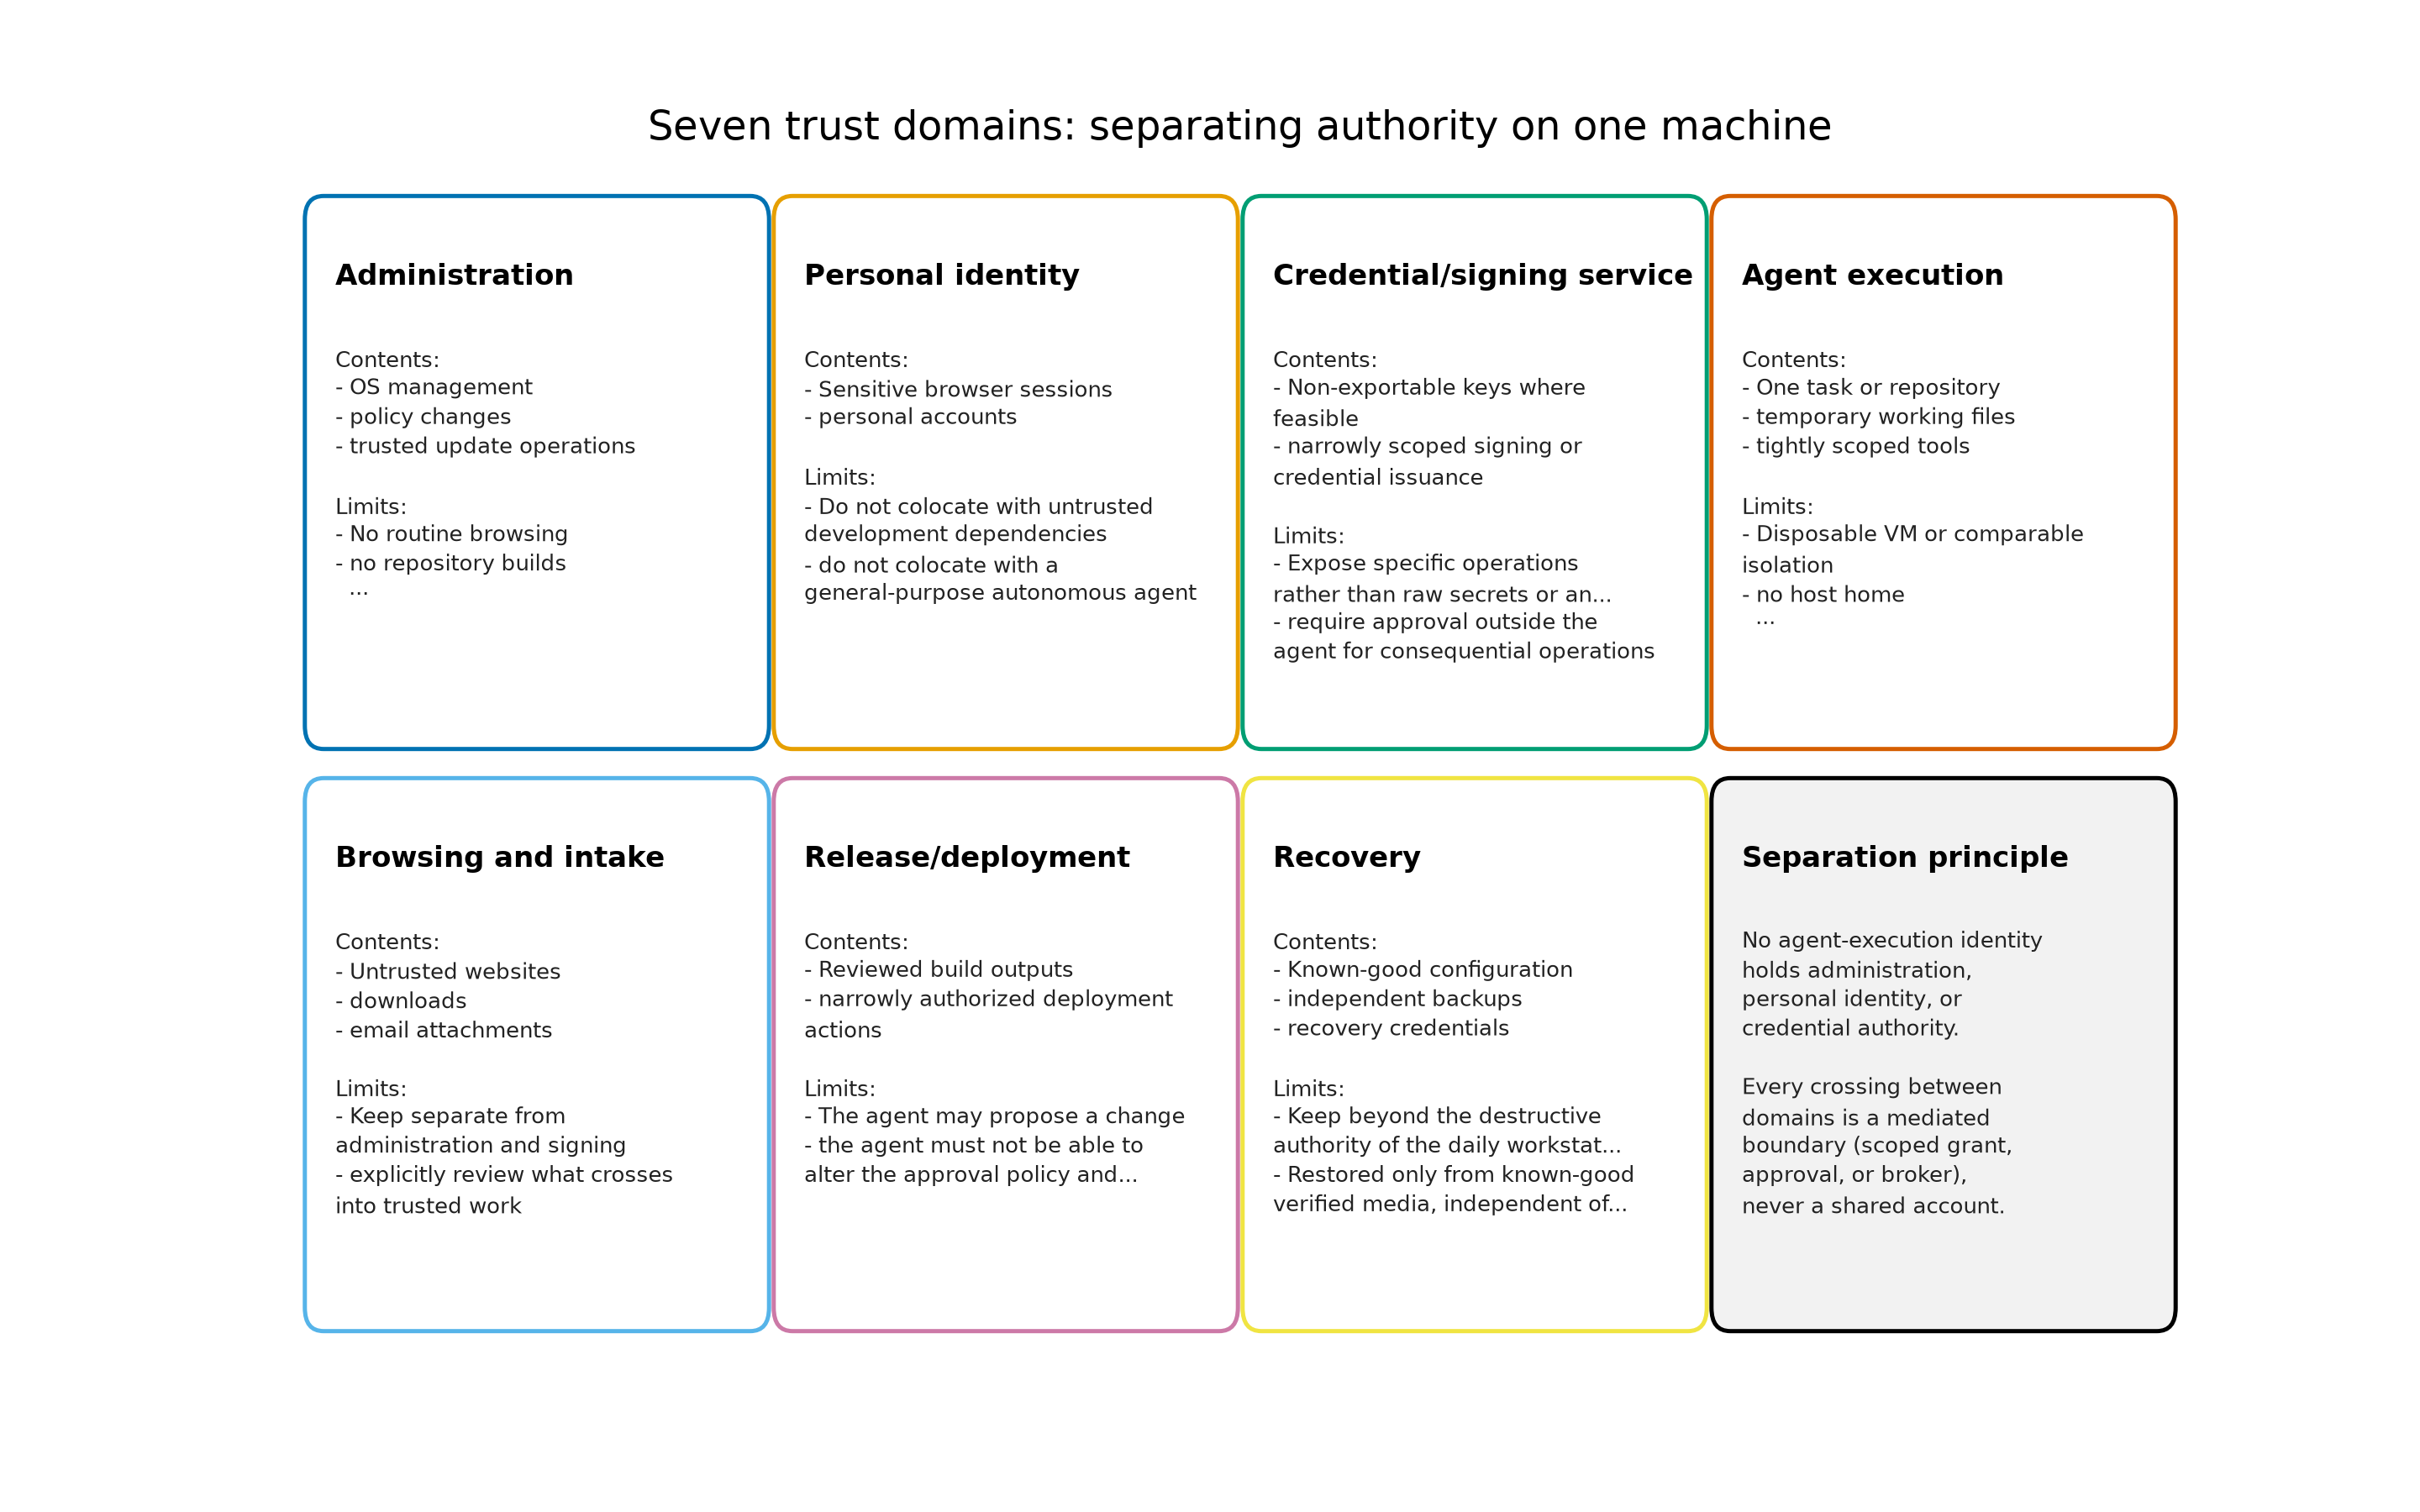
\includegraphics[width=1\linewidth,height=0.40\textheight,keepaspectratio,alt={Seven trust domains for AI-assisted work, arranged from hostile intake to protected assets; numbered arrows mark the control catalog entries that mediate each crossing.}]{../figures/trust_domains.png}
\caption{Seven trust domains for AI-assisted work, arranged from hostile
intake to protected assets; numbered arrows mark the control catalog
entries that mediate each crossing.}\label{fig:trust_domains}
\end{figure}

\end{frame}

\begin{frame}[allowframebreaks]{Seven trust domains}
The table and fig.~\ref{fig:trust_domains} encode two design judgments.
First, hostile-input domains and authority domains are different kinds
of places: agent execution and browsing/intake are deliberately cheap to
destroy, while administration, identity, and credentials are
deliberately expensive to enter. Second, the mapping onto concrete
platforms varies --- for a Qubes deployment these roles become a
manageable number of qubes with narrow qrexec policies (Project 2026b,
2026a); for a conventional workstation the highest-risk execution moves
to the separate VM host or machine described in sec.~8.
The objective in both cases is the same: real separation of authority,
not a diagram with many boxes.
\end{frame}

\begin{frame}[allowframebreaks]{Nine controls and their design
rationale}
\protect\phantomsection\label{nine-controls-and-their-design-rationale}
The domains define where authority lives; the controls define how work
crosses the boundaries. Each control below is stated as an operating
rule with the design rationale that makes it non-negotiable. Where a
shipping agent tool already implements a version of a rule, the
rationale cites the documented implementation --- as mechanism evidence,
not as an endorsement of any tool's security. The nine are also a
composed defense rather than a stack of independent toggles: Defense
Composition Algebra treats layered controls as formal objects whose
composition --- coverage interactions included, not just their count ---
determines what an attacker must defeat (Friedman 2026). In its notation
((\textbf{def:defense\_composition?})), a defense over the eight
mitigation classes is a composition of per-class layers, written as in
\end{frame}

\begin{frame}[allowframebreaks]{Nine controls and their design
rationale}
eq.~\ref{eq:defense_composition}, and the set below is chosen so that
each control closes a failure the others leave open.

\protect\phantomsection\label{def:defense_composition}
Layered controls compose over the eight mitigation classes as a single
formal object whose coverage interactions --- not merely the count of
layers --- determine what an attacker must defeat:
\begin{equation}\protect\phantomsection\label{eq:defense_composition}{D = d_1 \circ d_2 \circ \cdots \circ d_8}\end{equation}

\end{frame}

\begin{frame}[allowframebreaks]{Nine controls and their design
rationale}
\begin{longtable}[]{@{}
  >{\raggedright\arraybackslash}p{(\linewidth - 4\tabcolsep) * \real{0.3333}}
  >{\raggedright\arraybackslash}p{(\linewidth - 4\tabcolsep) * \real{0.3333}}
  >{\raggedright\arraybackslash}p{(\linewidth - 4\tabcolsep) * \real{0.3333}}@{}}
\caption{The nine controls of the agentic authority architecture:
operating rule and design rationale for each. The rules hold regardless
of host distribution; the rationales connect each control to a failure
it prevents, and where shipping agent tools implement a version of the
rule, the rationale points at the documented
mechanism.}\label{tbl:controls}\tabularnewline
\toprule\noalign{}
\begin{minipage}[b]{\linewidth}\raggedright
Control
\end{minipage} & \begin{minipage}[b]{\linewidth}\raggedright
Operating rule
\end{minipage} & \begin{minipage}[b]{\linewidth}\raggedright
Design rationale
\end{minipage} \\
\midrule\noalign{}
\endfirsthead
\toprule\noalign{}
\begin{minipage}[b]{\linewidth}\raggedright
Control
\end{minipage} & \begin{minipage}[b]{\linewidth}\raggedright
Operating rule
\end{minipage} & \begin{minipage}[b]{\linewidth}\raggedright
Design rationale
\end{minipage} \\
\midrule\noalign{}
\endhead
\textbf{Task-scoped credentials} & Prefer short-lived, repository- or
service-specific credentials; never hand the agent the owner's general
cloud identity because a task occasionally needs a deployment. & An
agent can only misuse authority it holds. Scoping bounds the
authorized-misuse blast radius at issuance time, which is the last
moment the choice is fully under the principal's control. \\
\textbf{Boundary-controlled egress} & Allow only required destinations,
at a boundary the agent cannot rewrite, and account for permitted
destinations that themselves accept uploads or messages. & A hostname
allowlist is not a data-loss policy: issue trackers, paste sites, CI
logs, and webhooks are all ``allowed hosts'' that exfiltrate. Egress
control must govern channels, not merely names. Shipping implementations
confirm the mechanism is standard --- Claude Code routes sandbox network
access through a proxy that enforces an allowed-domains list, and
documents the caveats: the proxy mediates by host, dynamic DNS and
request-URL discrepancies need explicit attention, and allowed sites
that accept arbitrary uploads remain channels (Anthropic 2026b); Codex
disables network access by default in its workspace-write mode and
requires it to be enabled per policy (OpenAI 2026). Neither mechanism
converts a hostname allowlist into a data-loss policy, which is why the
control governs channels first. \\
\textbf{External approvals} & Require an independent human or
deterministic policy check for production changes, secret access,
account administration, and publishing. & A second AI instance reading
the same hostile material is not automatically an independent security
boundary: shared context material and correlated failure modes mean the
``reviewer'' can be persuaded by the same bytes. Independence must come
from different information and authority, not from a second instance.
Shipping approval mechanics confirm the rule's shape: agent tools expose
explicit permission modes --- default-prompt, accept-edits, plan, and
dangerous bypass variants --- where the default remains asking the user
before consequential action, and Claude Code's auto mode adds a
classifier that judges whether a proposed action is safe enough to
proceed without asking (Anthropic 2026b, 2026a). A classifier at the
approval rung is an automation of triage, not a replacement for the
independent check the rung names. \\
\textbf{Operation mediation, not vague intentions} & Services expose
constrained operations --- ``sign this exact artifact for this release''
--- never ``use the signing key responsibly.'' Approval context includes
the artifact, destination, scope, and expiration. & Vague intentions are
unenforceable because nothing checks compliance against them. Mediated
operations give the approver a concrete object to accept or reject and
give the audit trail something to record; this is the confused-deputy
fix of (Hardy 1988) applied at the API surface. \\
\textbf{Minimal shared state} & Transfer only the files a task needs;
treat returned code, documents, and build artifacts as untrusted until
checked; never automatically promote an agent's home directory or
development image into a trusted environment. & Shared state is the
channel by which hostile content reaches authority. Every unreviewed
promotion is a boundary crossing performed by the agent rather than the
policy. \\
\textbf{Environment refresh} & Destroy task environments when work ends;
apply updates before creating the next ones. Distinguish deletion of an
environment from revocation of credentials it could access. & Refresh
caps how long a foothold persists, but deletion touches only the
environment: credentials already issued outlive it and must be revoked
on their own schedule. Conflating the two leaves live authority
attributed to a dead machine. \\
\textbf{Tool-bridge constraining} & Review filesystem, browser,
repository, CI, cloud, and messaging integrations as explicit grants of
authority, scoped like any other credential. & An isolated process with
a powerful API token is still a powerful actor: the tool bridge is where
isolation boundaries and API authority meet, and unreviewed bridges are
the agent-era equivalent of an unconfined daemon holding a root key. \\
\textbf{Independent audit trail} & Record tool use, permission grants,
policy changes, and deployment decisions outside the execution
environment; make the record sufficient to reconstruct what happened. &
The record must survive the thing being audited and must capture
actions, not agent prose. An audit trail inside the environment the
agent controls is a draft the agent can edit. \\
\textbf{Rehearsed recovery} & Test rebuilding the environment, revoking
credentials, recovering keys, and restoring data --- before the
incident. Assume a rebuild cannot undo data already exfiltrated or
remote changes already accepted. & Recovery rehearsal converts a
theoretical plan into a measured capability. Its honest limit is
temporal: restoration acts on the future; exfiltration and accepted
remote changes are in the past and are addressed only by revocation and
downstream containment. \\
\bottomrule\noalign{}
\end{longtable}

\end{frame}

\begin{frame}[allowframebreaks]{Nine controls and their design
rationale}
Two further trust-boundary decisions concern the models themselves. For
\textbf{local inference}, compute is not authority: do not attach
sensitive credentials to an inference environment merely because it
needs substantial GPU resources. A reasonable design separates the model
service from agent execution and from credential mediation, with
explicit authentication between them --- the model service is a
component, not a trusted co-resident. For \textbf{hosted models}, the
decision to transmit private code, documents, or credentials to a
provider is an independent trust-boundary decision that no
operating-system choice resolves: it determines who else processes the
material, under what retention, under which jurisdiction. Both decisions
sit above the host-distribution comparisons of sec.~5,
sec.~6, and sec.~7; neither can be
settled by switching distributions.
\end{frame}

\begin{frame}[fragile,allowframebreaks]{Convergent implementations in
shipping agent tools}
\protect\phantomsection\label{convergent-implementations-in-shipping-agent-tools}
The controls above are sometimes read as a bespoke architecture this
review invented. The engineering record says otherwise: three widely
deployed coding agents converge on the same primitive set, assembled
differently per platform, from a single policy model.

Claude Code documents a filesystem sandbox built on bubblewrap on Linux
and Seatbelt on macOS, network access mediated by a proxy that enforces
an allowed-domains list, and approval machinery in which every command
defaults to asking the user, with explicit modes for accepting edits and
a classifier-driven auto mode for lower-risk flows; its documentation
also names the allowlist's limits --- host-level mediation, DNS
dynamics, sites that accept uploads --- rather than overstating what a
domain list buys (Anthropic 2026b, 2026a). Codex documents the same
\end{frame}

\begin{frame}[fragile,allowframebreaks]{Convergent implementations in
shipping agent tools}
convergence from the policy-model side: one \texttt{SandboxPolicy}
compiles to Seatbelt on macOS, to bubblewrap and Landlock on Linux, and
to Windows DACL/appcontainer mechanisms, with mode presets (read-only,
workspace-write, danger-full-access) and network off by default in the
write modes (OpenAI 2026). Gemini CLI ships configurable sandboxing
across Seatbelt, Docker, gVisor, and bubblewrap backends on its
supported platforms (Google 2026). The pattern is the point: three
independent vendors, one shared conclusion that agent containment is
assembled from the same kernel-level primitives --- namespace and
MAC-framework sandboxing on the filesystem axis, a mediation point on
the network axis, and an approval or classifier layer on the decision
axis --- that the server candidates of sec.~8 expose as
ordinary configuration. The convergence also marks the frontier of the
architecture: none of these mechanisms, as documented, includes the
\end{frame}

\begin{frame}[fragile,allowframebreaks]{Convergent implementations in
shipping agent tools}
credential-scoping or audit controls of this section, which is exactly
the gap the trust-domain design addresses.

The convergence has a design consequence the rationales above now state
explicitly. Because the primitives are shared, an operator can evaluate
any agent-sandbox claim directly: which filesystem mechanism
(bubblewrap, Seatbelt, Landlock), whether egress is proxy-mediated or
merely filtered, whether the network default is closed, and which
approvals remain outside the agent. Vague answers to those four
questions identify an agent whose containment is a convenience, not a
boundary.
\end{frame}

\begin{frame}[allowframebreaks]{The authority ladder}
\protect\phantomsection\label{the-authority-ladder}
\end{frame}

\begin{frame}[allowframebreaks]{The authority ladder}
\begin{figure}
\centering
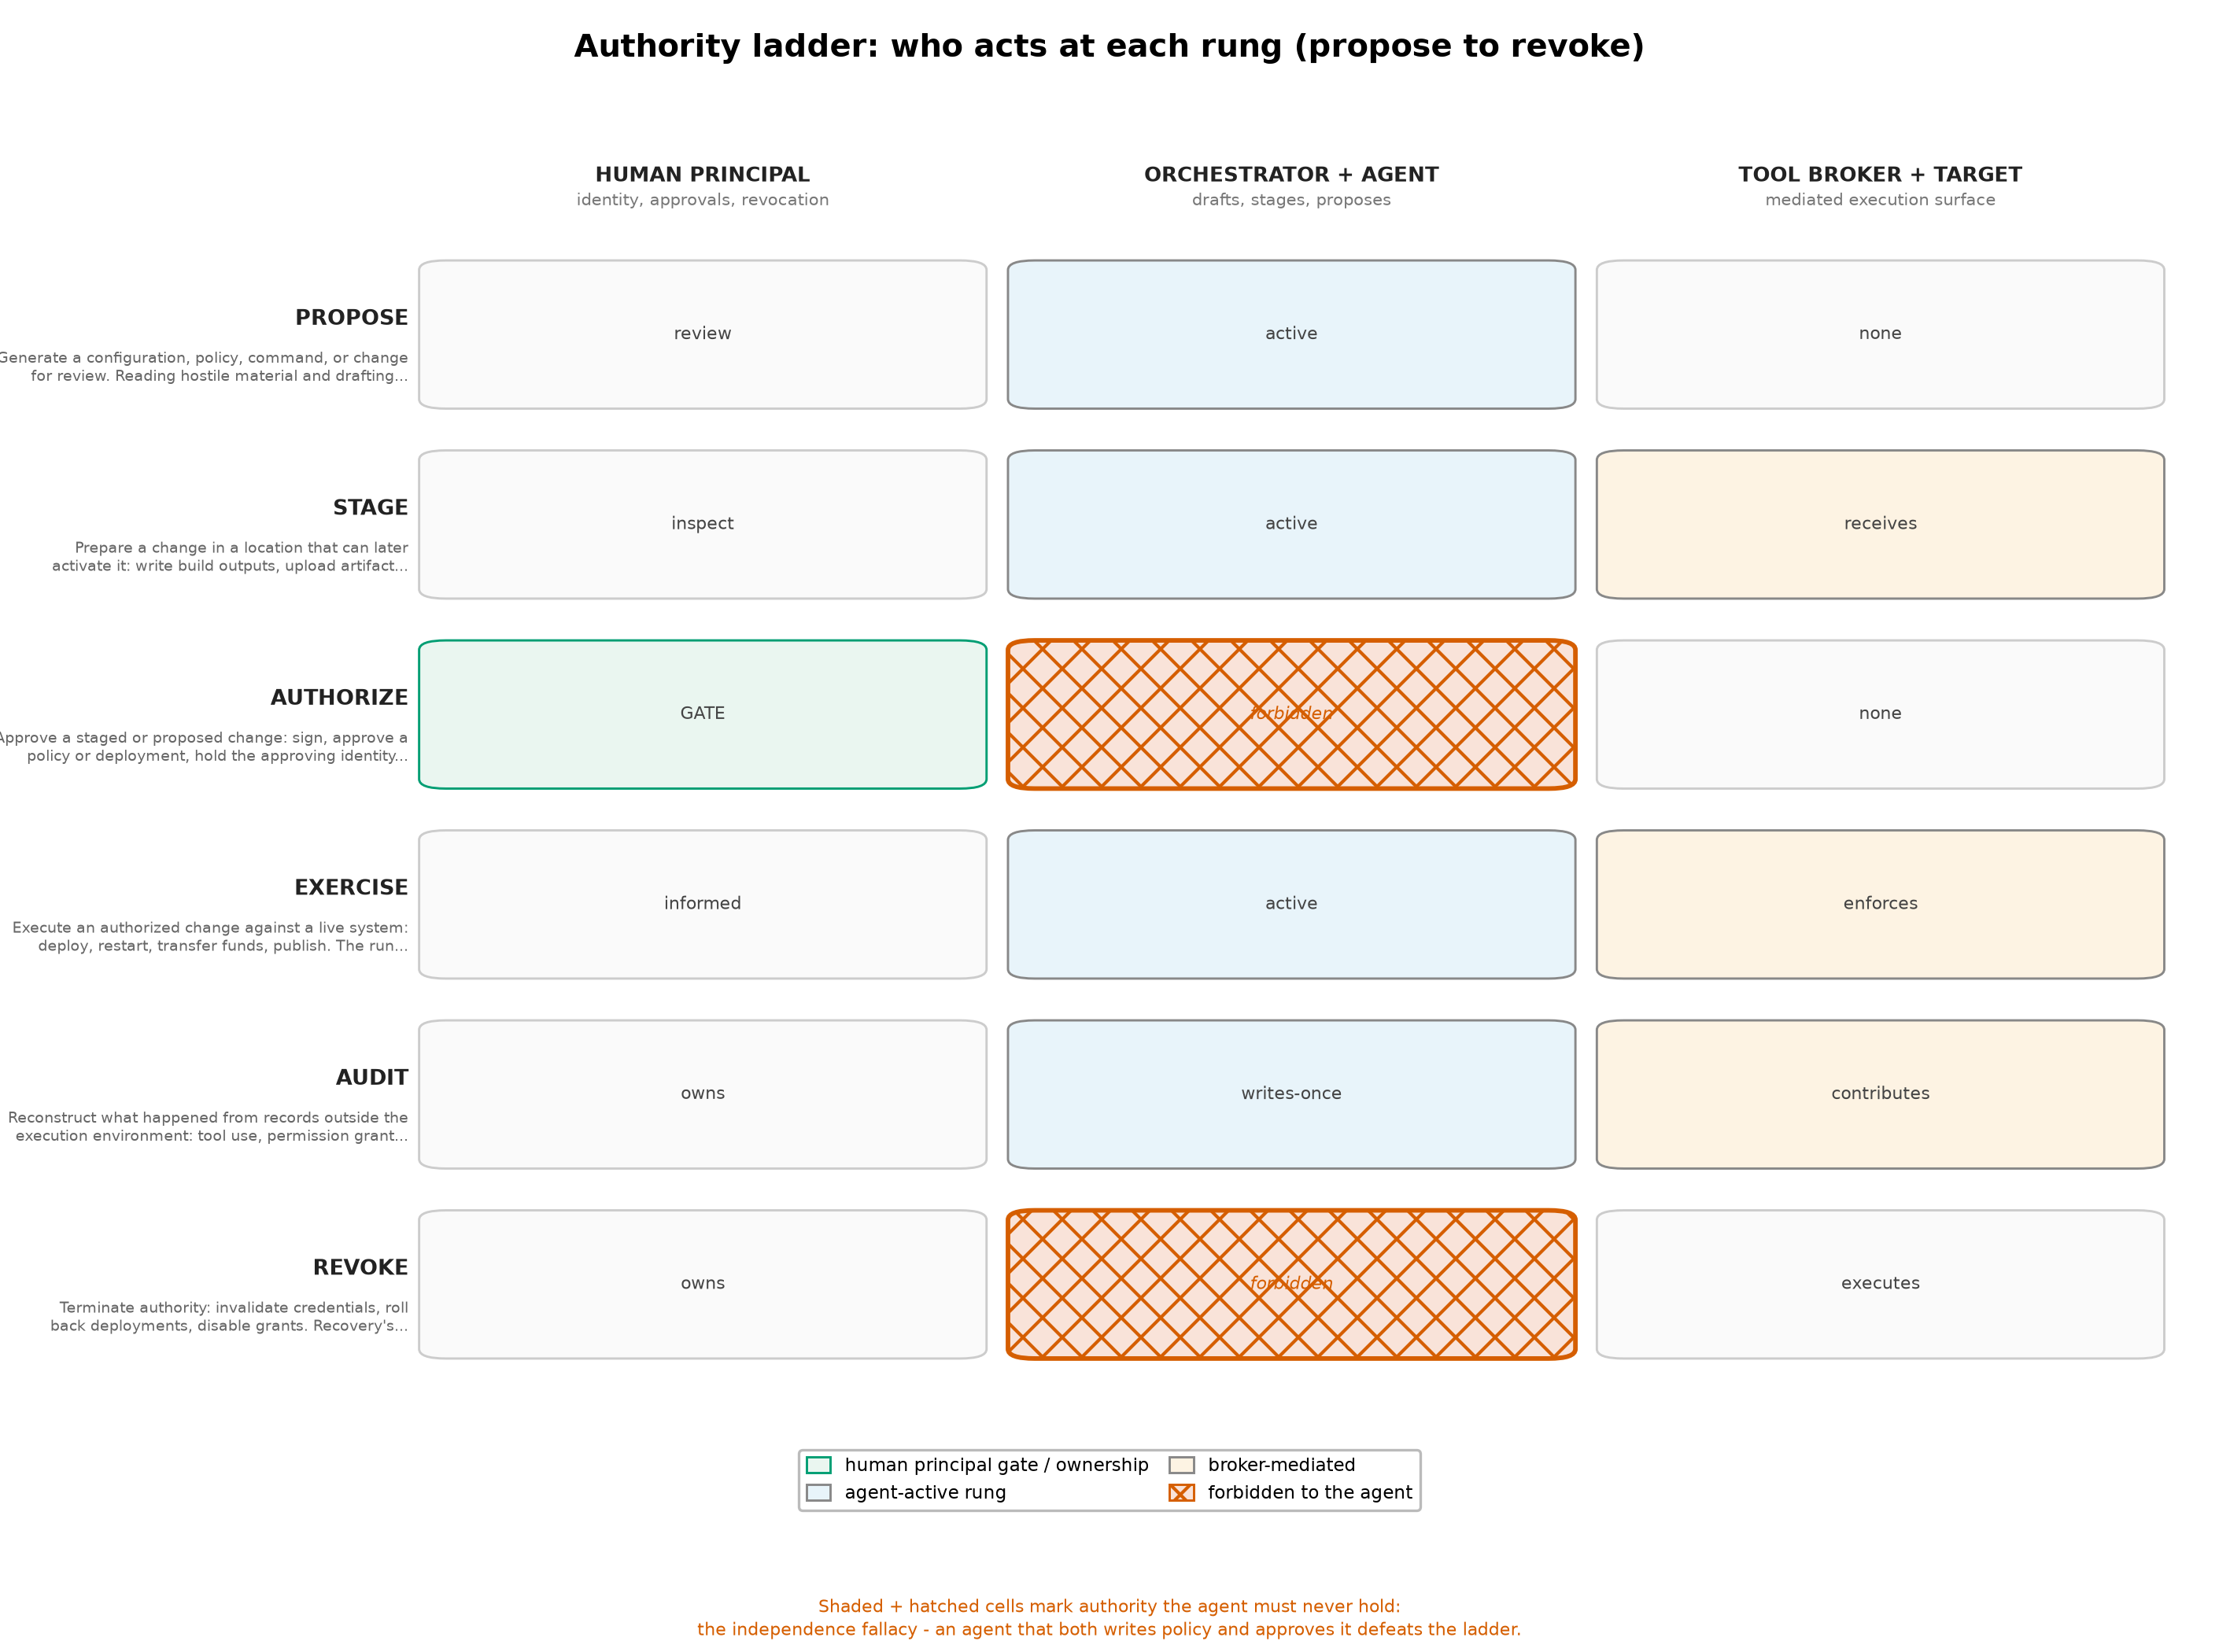
\includegraphics[width=1\linewidth,height=0.40\textheight,keepaspectratio,alt={The six-rung authority ladder as a swimlane across human principal, orchestrator and agent, and tool broker; hatched cells mark exercise paths an agent must never hold without external authorization.}]{../figures/authority_ladder.png}
\caption{The six-rung authority ladder as a swimlane across human
principal, orchestrator and agent, and tool broker; hatched cells mark
exercise paths an agent must never hold without external
authorization.}\label{fig:authority_ladder}
\end{figure}

\end{frame}

\begin{frame}[allowframebreaks]{The authority ladder}
The ladder in fig.~\ref{fig:authority_ladder} gives the architecture its
operating rhythm across six rungs: \textbf{propose}, \textbf{stage},
\textbf{authorize}, \textbf{exercise}, \textbf{audit}, \textbf{revoke},
ordered as in eq.~\ref{eq:authority_ladder_order}. An agent may propose
and stage freely --- generating configurations, preparing artifacts,
drafting deployments --- because nothing at those rungs changes the
world. Authorization is the hinge: it must be exercised outside the
agent, by the human principal or by deterministic policy, and the
approval context is a mediated operation with artifact, destination,
scope, and expiration. Exercise happens under whatever scopes the
authorization granted, no more. Audit and revoke are not afterthoughts
but standing rungs: the audit record lives outside the execution
environment so it survives the environment's destruction, and revocation
\end{frame}

\begin{frame}[allowframebreaks]{The authority ladder}
is the only rung that addresses what a rebuild cannot --- authority
already exercised against the outside world. An architecture that lets
the agent climb from propose to authorize on its own has not built a
ladder; it has built a loop, and the configuration-side invariants that
prevent exactly that are specified and enforced in
sec.~14. The permission modes of the
shipping tools read as partial ladders: default-prompt modes place
authorize with the human; accept-edits moves routine edit-authorization
to the agent while keeping command approval; bypass modes remove the
hinge altogether and are, in this architecture's terms, a design
admission rather than a mode (Anthropic 2026b; OpenAI 2026).

\end{frame}

\begin{frame}[allowframebreaks]{The authority ladder}
The authorize/exercise split of (\textbf{def:authority\_ladder\_order?})
is also what keeps delegated trust bounded, and it has a
commercial-integrity ancestry: Clark and Wilson grounded integrity in
well-formed transactions, in which data changes state only through a
mediated operation whose form is certified in advance, and in separation
of duty, which prevents the principal who certifies an operation from
being the one who executes it (Clark and Wilson 1987). Operation
mediation and the approve/exercise split of this section are those
controls restated for agents. Formal treatments of agent trust bound a
delegate's effective trust by what it was authorized to exercise rather
than by what it can reach, and the ladder encodes that bound
structurally: authorization fixes the scope, exercise consumes it, and
no rung is reachable that lets the agent enlarge its own authorization
(Friedman 2026). The orchestration section extends the same bound across
\end{frame}

\begin{frame}[allowframebreaks]{The authority ladder}
agent-to-agent delegation chains, where unbounded trust would otherwise
amplify with each hop sec.~13.

The trust domains, controls, and ladder compose into the scenarios of
sec.~16: a Qubes deployment realizes the domains as
qubes with narrow communication policies (Project 2026b), a conventional
workstation realizes them through the separate execution infrastructure
of sec.~8, and the orchestration layer realizes the
ladder over fleets as described in sec.~13. The
operator behaviors that keep the separation real --- and the cognitive
failure modes that erode it --- are the subjects of sec.~12
and sec.~11.
\end{frame}

\end{document}
